\documentclass[11pt,a4paper]{article}

\usepackage[utf8]{inputenc}
\usepackage[T1]{fontenc}
\usepackage{lmodern}
\usepackage[margin=2.35cm,headheight=15pt]{geometry}
\usepackage{amsmath,amssymb,bm}
\usepackage{graphicx}
\usepackage{booktabs,longtable,array}
\usepackage{xcolor}
\usepackage{listings}
\usepackage{hyperref}
\usepackage{xurl}
\usepackage{caption}
\usepackage{float}
\usepackage{placeins}
\usepackage{fancyhdr}
\usepackage{microtype}
\usepackage{enumitem}
\usepackage{subcaption}

\definecolor{codebg}{RGB}{246,247,249}
\definecolor{codeframe}{RGB}{210,214,220}
\definecolor{codeblue}{RGB}{28,75,130}
\definecolor{codegreen}{RGB}{35,115,75}
\hypersetup{
  colorlinks=true,
  linkcolor=codeblue,
  urlcolor=codeblue,
  citecolor=codegreen,
  pdftitle={ROOT Phase-Space Monte Carlo Tutorial},
  pdfauthor={Supernova Graviton MC project}
}
\lstdefinestyle{terminal}{
  basicstyle=\ttfamily\small,
  backgroundcolor=\color{codebg},
  frame=single,
  rulecolor=\color{codeframe},
  breaklines=true,
  columns=fullflexible,
  keepspaces=true,
  showstringspaces=false,
  upquote=true,
  xleftmargin=0.5em,
  xrightmargin=0.5em,
  aboveskip=0.7em,
  belowskip=0.7em
}
\lstset{style=terminal}

\pagestyle{fancy}
\fancyhf{}
\lhead{Supernova Graviton MC}
\rhead{Technical Tutorial}
\cfoot{\thepage}
\setlength{\parskip}{0.35em}
\setlength{\parindent}{0pt}
\setlist[itemize]{leftmargin=1.6em,itemsep=0.2em,topsep=0.3em}
\setlist[enumerate]{leftmargin=1.8em,itemsep=0.2em,topsep=0.3em}
\setcounter{tocdepth}{1}

\newcommand{\dd}{\,\mathrm{d}}
\newcommand{\M}{\mathcal{M}}
\newcommand{\ee}{e^-}
\newcommand{\ep}{e^+}
\newcommand{\hgr}{h}
\newcommand{\code}[1]{\texttt{\detokenize{#1}}}
\newcommand{\GeV}{\,\mathrm{GeV}}
\newcommand{\MeV}{\,\mathrm{MeV}}

\title{\vspace{-1.1cm}\textbf{ROOT Phase-Space Monte Carlo for Thermal Graviton Production in Supernova Cores}\\[0.4em]
\large Technical Tutorial}
\author{Supernova Graviton MC project}
\date{October 2026}

\begin{document}
\maketitle
\thispagestyle{fancy}

\begin{abstract}
This document is a technical manual for the C++/ROOT implementation used to construct phase-space event pools and evaluate channel-specific thermal graviton spectra in a supernova-core profile. It focuses on repository layout, input conventions, importance sampling, phase-space generation, event reweighting, numerical output, and practical commands. The five channel-level analytical/Monte Carlo comparison plots are included as implementation checks. Detailed amplitude derivations and the interpretation of the combined physical spectrum belong in the associated paper and its Supplemental Material, not in this tutorial.
\end{abstract}

\tableofcontents
\newpage

\section{Purpose and scope}

The code evaluates thermal graviton production for five microscopic channels:
\begin{align*}
\gamma e^- &\to h e^-, & \gamma p &\to h p,\\
e^-e^+ &\to h\gamma, & e^-Z &\to h e^-Z,\\
e^-e^- &\to h e^-e^-.
\end{align*}

The implementation follows a two-stage workflow. A generator samples local supernova conditions and initial-state momenta, then creates on-shell final-state kinematics and writes a reusable ROOT event pool. A separate reweighter reads that pool, evaluates the channel-specific matrix element and thermal factors, and accumulates the spectrum in logarithmic graviton-energy bins.

\begin{center}
\fbox{\parbox{0.91\linewidth}{\centering
\textbf{Profile CSV} $\;\to\;$ \textbf{thermal proposal} $\;\to\;$ \textbf{ROOT phase space} $\;\to\;$ \textbf{event reweighting} $\;\to\;$ \textbf{spectrum CSV}
}}
\end{center}

\textbf{Scope boundary.} ROOT handles the event kinematics and phase-space proposal. The calculation still uses channel-dependent physics approximations, including massless-electron limits in selected channels, leading-soft bremsstrahlung kernels, and Debye screening prescriptions. Exact kinematics should not be interpreted as an exact finite-temperature QFT calculation.

\section{Repository layout}

The tutorial assumes that it is placed in the repository's \code{docs/} directory and that the source and input files use the following layout:

\begin{lstlisting}
.
|-- data/
|   |-- sn_profile_data.csv
|   `-- sn_profile_data_muInc.csv
|-- src/
|   |-- generate_gammae_phsp.cpp
|   |-- weight_gammae_spectrum.cpp
|   |-- generate_gammap_phsp.cpp
|   |-- weight_gammap_spectrum.cpp
|   |-- generate_eann_phsp.cpp
|   |-- weight_eann_spectrum.cpp
|   |-- generate_brem_phsp_v1.cpp
|   `-- weight_brem_spectrum_v1.cpp
`-- docs/
    |-- ROOT_PHSP_Tutorial.tex
    |-- ROOT_PHSP_Tutorial.pdf
    `-- figures/
        |-- gammae_analytical_mc.png
        |-- gammap_analytical_mc.png
        |-- eann_analytical_mc.png
        |-- ez_analytical_mc.png
        `-- ee_analytical_mc.png
\end{lstlisting}

The filenames above correspond to the code snapshot documented here. If source filenames or profile schemas change in the repository, update the commands and this document together.

\section{Requirements and build}

\subsection{Software}

\begin{itemize}
  \item A ROOT installation with \code{root-config}. The programs use ROOT classes including \code{TFile}, \code{TTree}, \code{TLorentzVector}, and \code{TGenPhaseSpace}.
  \item A C++ compiler with C++17 support.
  \item A shell environment in which the ROOT setup script has been sourced.
\end{itemize}

Check the environment before compiling:

\begin{lstlisting}[language=bash]
root-config --version
root-config --cflags
root-config --libs
\end{lstlisting}

Build all eight programs from the repository root:

\begin{lstlisting}[language=bash]
mkdir -p build output

for name in \
  generate_gammae_phsp weight_gammae_spectrum \
  generate_gammap_phsp weight_gammap_spectrum \
  generate_eann_phsp weight_eann_spectrum \
  generate_brem_phsp_v1 weight_brem_spectrum_v1
do
  g++ -O3 -std=c++17 "src/${name}.cpp" \\
      $(root-config --cflags --libs) \\
      -o "build/${name}" || exit 1
done
\end{lstlisting}

The build command links each executable against ROOT. No separate plotting library is required by the C++ programs; the reweighters write CSV files.

\section{Input profiles and local thermodynamic quantities}

\subsection{Profile files}

\code{data/sn_profile_data.csv} contains four columns, in this order:

\begin{center}
\begin{tabular}{ll}
\toprule
Column & Meaning \\
\midrule
\code{r_km} & Radius in km \\
\code{rho_g_cm3} & Mass density in g cm$^{-3}$ \\
\code{Yp} & Proton fraction \\
\code{T_MeV} & Temperature in MeV \\
\bottomrule
\end{tabular}
\end{center}

The parser accepts comma-separated or whitespace-separated rows and skips non-numeric header lines. The annihilation generator uses \path{data/sn_profile_data_muInc.csv}, which adds \path{mu_old_GeV} and \path{mu_precise_GeV}. In that file, \path{mu_old_GeV} is the zero-temperature Fermi-momentum estimate used for the density normalization, while \path{mu_precise_GeV} is the finite-temperature charge-neutrality solution used in the electron/positron distributions.

\subsection{Sampling radius and interpolation}

For a requested outer radius $R$, the generator samples
\begin{equation}
  r = R u^{1/3}, \qquad u\sim\mathcal{U}(0,1),
\end{equation}
which is uniform in physical volume, since $\dd V=4\pi r^2\dd r$. The tabulated profile is linearly interpolated in radius. The default value of $R$ in the executables is $18\,\mathrm{km}$; it can be overridden by the final command-line argument.

For the photoproduction and bremsstrahlung profiles, the current implementation obtains the proton/electron density scale from
\begin{equation}
 n_p\simeq n_e = \frac{\rho Y_p}{m_N}, \qquad
 \mu_e\simeq (3\pi^2 n_e)^{1/3},
\end{equation}
with the conversion from g cm$^{-3}$ to natural units performed in the source. The Debye momentum used by these channels follows the code convention
\begin{equation}
 \kappa^2 = \frac{8\pi\alpha n_e}{T},
\end{equation}
corresponding to the working approximation $n_p\simeq n_e$. The annihilation channel instead reads its refined finite-temperature chemical potential from the dedicated profile.

\section{Monte Carlo architecture}

\subsection{Importance sampling of initial states}

The initial-state proposals are chosen to cover the physically relevant distributions efficiently. They are not themselves the physical distributions. Each reweighter computes an event-by-event proposal correction, schematically
\begin{equation}
 R_a(p) = \frac{q_{a,\mathrm{phys}}(p)}{g_a(p)},
\end{equation}
where $g_a$ is the normalized proposal density used by the generator and $q_{a,\mathrm{phys}}$ is the normalized radial momentum density associated with the physical occupation function. The density normalization is applied separately in the rate prefactor.

The current source uses the following proposals:
\begin{itemize}
  \item \textbf{$\gamma e$ photoproduction:} the electron momentum magnitude is sampled uniformly on $[0,\mu_e+15T]$; the photon uses a broad exponential proposal with scale $10T$. The event weight restores the momentum dependence used by the reweighter.
  \item \textbf{$\gamma p$ photoproduction:} the proton follows a nonrelativistic Maxwell distribution. The photon proposal is a mixture of a nominal thermal-shaped component and a broader high-energy component; the mixture ratio is corrected event by event.
  \item \textbf{$e^-e^+$ annihilation:} the electron proposal covers the degenerate Fermi-sea region and a thermal tail. The positron radial proposal has a Gamma distribution with shape $k=3$ and scale $T$. The code uses $\mu_{e^+}=-\mu_{e^-}$.
  \item \textbf{$ee$ and $eZ$ bremsstrahlung:} full-support thermal proposals are used, including components that improve sampling near the electron Fermi surface and in the tails. Proposal densities are stored in the ROOT pool and divided out in the reweighting stage.
\end{itemize}

\subsection{Final-state phase space with ROOT}

For each event, the incoming four-momenta are defined in the local plasma rest frame and summed to form the parent four-vector
\begin{equation}
 P^\mu = p_1^\mu+p_2^\mu.
\end{equation}
The generator passes $P^\mu$ and the final-state masses to ROOT's \code{TGenPhaseSpace}. ROOT generates on-shell two-body kinematics for the photoproduction and annihilation channels, and three-body kinematics for bremsstrahlung. The generated four-vectors are stored in the plasma frame, so the graviton energy used for the spectrum is $\omega=k_h^0$ in that frame.

The phase-space correction stored in the tree is channel dependent:
\begin{itemize}
  \item $\gamma e$ and $e^-e^+\to h\gamma$: the two-body final state is massless in the implemented kinematics, so the integrated two-body phase-space factor is represented by the constant $1/(8\pi)$ in the reweighter.
  \item $\gamma p$: the massive-proton recoil changes the two-body phase space; the generator stores the corresponding $w_{\Phi_2}$ correction.
  \item $ee$ and $eZ$: the generator stores a three-body phase-space/proposal correction $w_{\Phi_3}$, which is included by the reweighter.
\end{itemize}

The phase-space pool is therefore a reusable set of integration points, not a list of unit-weight physical collisions. The matrix element, occupation factors, density prefactors, flux factor, blocking factors, and channel-specific statistical factors are applied in the weighting stage.

\subsection{Event weight and spectrum estimator}

For orientation, the structure of a weighted event can be written schematically as
\begin{equation}
 w_i = V\,n_a n_b\,R_aR_b\,
 \frac{1}{4E_aE_b}\,w_{\Phi_n}\,\overline{|\M_i|^2}\,
 B_{\mathrm{final}}\,S_{\mathrm{ident}}.
 \label{eq:event-weight}
\end{equation}
Here $V$ is the sampled core volume, $R_a$ and $R_b$ are proposal corrections, $w_{\Phi_n}$ is the channel-specific phase-space factor, $B_{\mathrm{final}}$ denotes final-state Pauli blocking where applicable, and $S_{\mathrm{ident}}$ denotes identical-particle factors where applicable. Equation~\eqref{eq:event-weight} is a schematic map of the code architecture; normalization details are channel-specific and are implemented in the source.

The spectrum is accumulated in logarithmic energy bins. For a bin of width $\Delta\ln\omega$, the estimator is
\begin{equation}
 \left(\omega\frac{\dd P}{\dd\omega}\right)_j
 = \frac{1}{N_{\mathrm{proposal}}\,\Delta\ln\omega}
   \sum_{i\in j}\omega_i w_i.
 \label{eq:spectrum-estimator}
\end{equation}
The sum is normalized by the number of generated proposals, not merely by the number of events that happen to land in a bin. The reweighters also accumulate the sum of squared contributions to estimate the Monte Carlo uncertainty and calculate an effective weighted event count,
\begin{equation}
 N_{\mathrm{eff},j}=\frac{(\sum_{i\in j}z_i)^2}{\sum_{i\in j}z_i^2},
 \qquad z_i=\omega_i w_i.
\end{equation}
A low raw count or low effective count in the far tail usually signals that more proposals are needed there; it does not by itself imply a failure of the matrix element.

\section{Channel-specific implementation conventions}

\small
\begin{longtable}{p{0.18\linewidth}p{0.72\linewidth}}
\toprule
Channel & Implementation conventions \\
\midrule
\endfirsthead
\toprule
Channel & Implementation conventions \\
\midrule
\endhead
$\gamma e\to he$ & Massless-electron kinematics. The reweighter evaluates the screened kernel using the invariant denominator $\kappa^2-t$, includes the outgoing-electron Pauli factor $1-f_e(E_{\mathrm{out}})$, and uses a constant massless two-body phase-space factor. \\
\addlinespace
$\gamma p\to hp$ & The initial proton is sampled nonrelativistically, but final-state proton recoil and the two-body phase space are retained. The matrix element is evaluated after boosting the incoming photon and outgoing graviton into the incoming-proton rest frame. Screening is included in the stable combined expression for the massive-proton kernel. \\
\addlinespace
$e^-e^+\to h\gamma$ & Uses the finite-temperature chemical potential \code{mu_precise_GeV}. The positron distribution uses the opposite chemical potential, $\mu_{e^+}=-\mu_{e^-}$. There is no final-state electron, so no electron Pauli-blocking factor appears. \\
\addlinespace
$eZ\to heZ$ & Leading-soft graviton emission from electron scattering on a static heavy source. In the current implementation the target has proton mass and charge $Z=1$. The squared-amplitude screening is $S_Q^2$, with $S_Q=Q^2/(Q^2+\kappa^2)$; it is implemented algebraically through the screened transfer denominator. \\
\addlinespace
$e^-e^-\to he^-e^-$ & Leading-soft graviton kernel multiplied by the screened M\o ller kernel. Screening is applied once at the squared-amplitude level as $S_tS_u$, where $S_t=(-t)/(\kappa^2-t)$ and $S_u=(-u)/(\kappa^2-u)$. Both initial- and final-state identical-electron factors, $1/2\times1/2=1/4$, are applied outside the squared amplitude by the reweighter. \\
\bottomrule
\end{longtable}
\normalsize

\subsection{Frame conventions}

\begin{center}
\begin{tabular}{p{0.36\linewidth}p{0.53\linewidth}}
\toprule
Quantity or operation & Frame/convention \\
\midrule
Thermal profiles, initial-state distributions, Pauli blocking & Local plasma rest frame \\
Graviton energy used for binning & Plasma rest frame, $\omega=k_h^0$ \\
ROOT phase-space construction & Parent rest frame internally; returned event four-vectors are boosted to the frame of the parent input \\
$\gamma p$ matrix element & Incoming-proton rest frame \\
$eZ$ bremsstrahlung kernel & Incoming-target rest frame / static-source approximation \\
$ee$ bremsstrahlung kernel & Invariants and soft products constructed from event four-vectors using the $(+,-,-,-)$ metric \\
\bottomrule
\end{tabular}
\end{center}



\section{Quick start: run \texorpdfstring{$\gamma e\to he$}{gamma e -> h e}}

This is the shortest end-to-end example. Run the commands from the repository root after building the executables:

\begin{lstlisting}[language=bash]
mkdir -p output

# Stage 1: generate a reusable ROOT event pool.
./build/generate_gammae_phsp \
  data/sn_profile_data.csv \
  output/gammae_phsp.root \
  5000000 20261024 18.0

# Stage 2: apply the physical weights and write the spectrum.
./build/weight_gammae_spectrum \
  output/gammae_phsp.root \
  output/gammae_spectrum.csv
\end{lstlisting}

The generator arguments are
\begin{center}
\code{profile.csv output.root Nproposal seed R_km}.
\end{center}
The weighting executable takes \code{input.root output.csv}. The number of proposals and seed are explicit in this example; changing the seed changes the Monte Carlo sample, while increasing \code{Nproposal} generally reduces statistical uncertainty.

\section{Commands for all channels}

The command-line interfaces are summarized below. All paths are relative to the repository root.

\subsection{Photon-electron photoproduction}

\begin{lstlisting}[language=bash]
./build/generate_gammae_phsp \
  data/sn_profile_data.csv output/gammae_phsp.root \
  5000000 20261024 18.0
./build/weight_gammae_spectrum \
  output/gammae_phsp.root output/gammae_spectrum.csv
\end{lstlisting}

\subsection{Photon-proton photoproduction}

\begin{lstlisting}[language=bash]
./build/generate_gammap_phsp \
  data/sn_profile_data.csv output/gammap_phsp.root \
  5000000 20261024 18.0
./build/weight_gammap_spectrum \
  output/gammap_phsp.root output/gammap_spectrum.csv
\end{lstlisting}

\subsection{Electron-positron annihilation}

\begin{lstlisting}[language=bash]
./build/generate_eann_phsp \
  data/sn_profile_data_muInc.csv output/eann_phsp.root \
  10000000 20261024 18.0
./build/weight_eann_spectrum \
  output/eann_phsp.root output/eann_spectrum.csv
\end{lstlisting}

\subsection{Bremsstrahlung: \texorpdfstring{$ee$ and $eZ$}{ee and eZ}}

The bremsstrahlung generator and reweighter share source files; select the channel with the first argument:

\begin{lstlisting}[language=bash]
# ee -> eeh
./build/generate_brem_phsp_v1 ee \
  data/sn_profile_data.csv output/ee_phsp.root \
  20000000 20261024 18.0
./build/weight_brem_spectrum_v1 ee \
  output/ee_phsp.root output/ee_spectrum.csv

# eZ -> eZh (current target: Z=1, proton mass)
./build/generate_brem_phsp_v1 ez \
  data/sn_profile_data.csv output/ez_phsp.root \
  20000000 20261024 18.0
./build/weight_brem_spectrum_v1 ez \
  output/ez_phsp.root output/ez_spectrum.csv
\end{lstlisting}

The generator argument order is \code{channel profile.csv output.root Nproposal seed R_km}; the reweighter argument order is \code{channel pool.root output.csv}. The event count above is an example, not a guarantee of the statistical precision shown in the figures. Production runs should use enough proposals to stabilize the bins of interest, especially the low-statistics tails.

\section{ROOT and CSV outputs}

\subsection{ROOT event pools}

The ROOT file contains an \code{events} tree with the initial and final four-vectors and local profile/proposal information required by the matching reweighter. It also stores metadata such as \code{N_PROPOSAL}, \code{N_VALID}, and \code{R_KM}. Branch names are channel-specific; inspect the corresponding generator if you add a new observable or change the event record.

The bremsstrahlung pool can exceed ROOT's per-tree file-size limit in large production runs. ROOT may then create sibling files such as \code{ee_phsp.root}, \code{ee_phsp_1.root}, and so on. The bremsstrahlung reweighter accepts the base filename and automatically chains the numbered siblings. Keep those files in the same directory and do not pass only one numbered fragment.

\subsection{Spectrum CSV}

The reweighters write the following columns:

\begin{center}
\small
\begin{tabular}{p{0.39\linewidth}p{0.50\linewidth}}
\toprule
Column & Meaning \\
\midrule
\path{omega_GeV} & Geometric center of the logarithmic $\omega$ bin \\
\path{omega_dP_domega_GeV2} & Estimate of $\omega\,\dd P/\dd\omega=\dd P/\dd\ln\omega$ \\
\path{mc_error_GeV2} & Estimated Monte Carlo standard error for the bin \\
\path{raw_event_count} & Number of accepted weighted events in the bin \\
\path{effective_weighted_events} & Effective count inferred from the first and second weight moments \\
\bottomrule
\end{tabular}
\normalsize
\end{center}

The binning limits are currently hard-coded in the reweighting sources. The $\gamma e$ reweighter uses 120 logarithmic bins from $8\times10^{-5}$ to $3.6\GeV$; the other channel reweighters use 180 bins from $8\times10^{-5}$ to $3.3\GeV$. To change the binning, edit the relevant \code{NBIN}, \code{omegaMin}, and \code{omegaMax} constants, then rebuild that reweighter.

\section{Channel-level analytical/MC checks}

The following five plots are the latest channel-specific comparison figures supplied for this tutorial. They are included as technical closure references only. No combined total-spectrum or channel-dominance overview is included here, to keep this document separate from the physical interpretation in the paper.

% ============================================================
% Photoproduction
% ============================================================
\begin{figure}[H]
  \centering

  \begin{subfigure}[t]{0.48\linewidth}
    \centering
    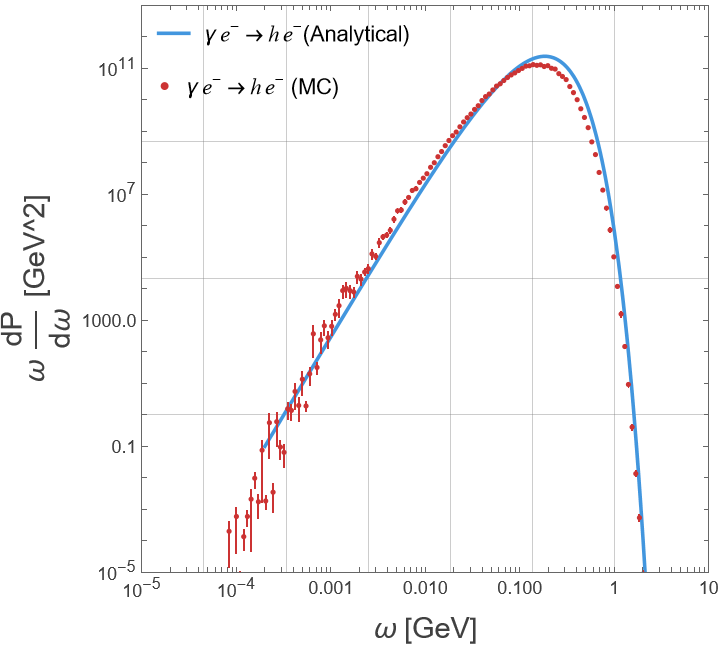
\includegraphics[width=\linewidth]{figures/gammae_analytical_mc.png}
    \caption{}
    \label{fig:gammae}
  \end{subfigure}
  \hfill
  \begin{subfigure}[t]{0.48\linewidth}
    \centering
    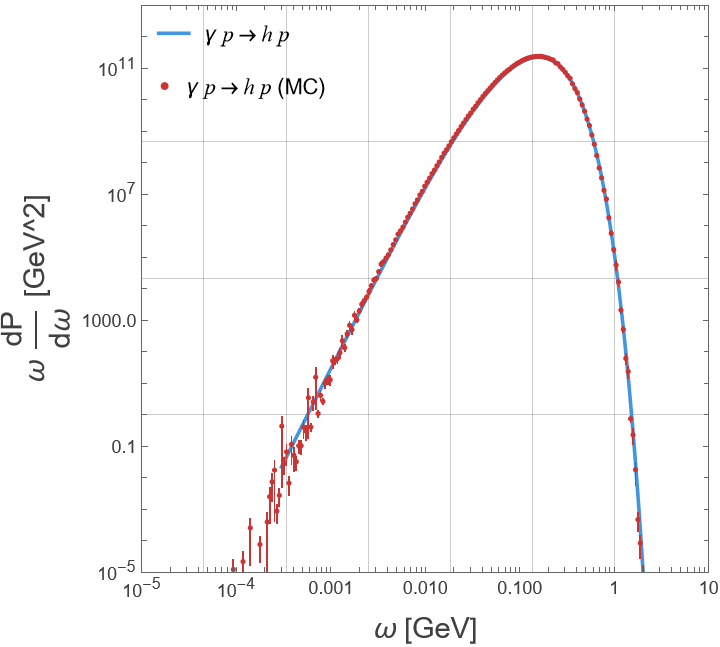
\includegraphics[width=\linewidth]{figures/gammap_analytical_mc.png}
    \caption{}
    \label{fig:gammap}
  \end{subfigure}

  \caption{
    Analytical and ROOT Monte Carlo results for graviton photoproduction:
    (a) electron photoproduction,
    $\gamma e^- \to h e^-$;
    (b) proton photoproduction,
    $\gamma p \to h p$.
    The points show the Monte Carlo spectra with statistical uncertainties,
    while the solid curves show the corresponding analytical results.
  }
  \label{fig:photoproduction_validation}
\end{figure}
\FloatBarrier


% ============================================================
% Bremsstrahlung
% ============================================================
\begin{figure}[H]
  \centering

  \begin{subfigure}[t]{0.48\linewidth}
    \centering
    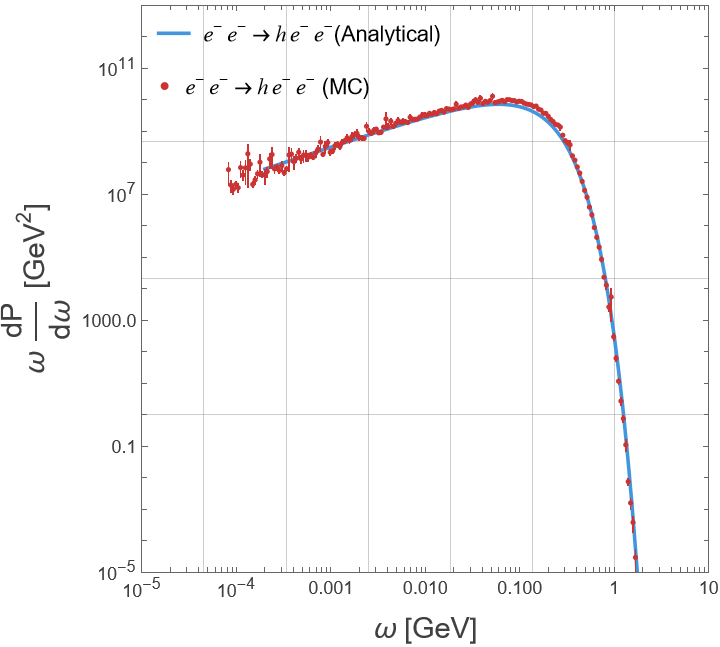
\includegraphics[width=\linewidth]{figures/ee_analytical_mc.png}
    \caption{}
    \label{fig:ee}
  \end{subfigure}
  \hfill
  \begin{subfigure}[t]{0.48\linewidth}
    \centering
    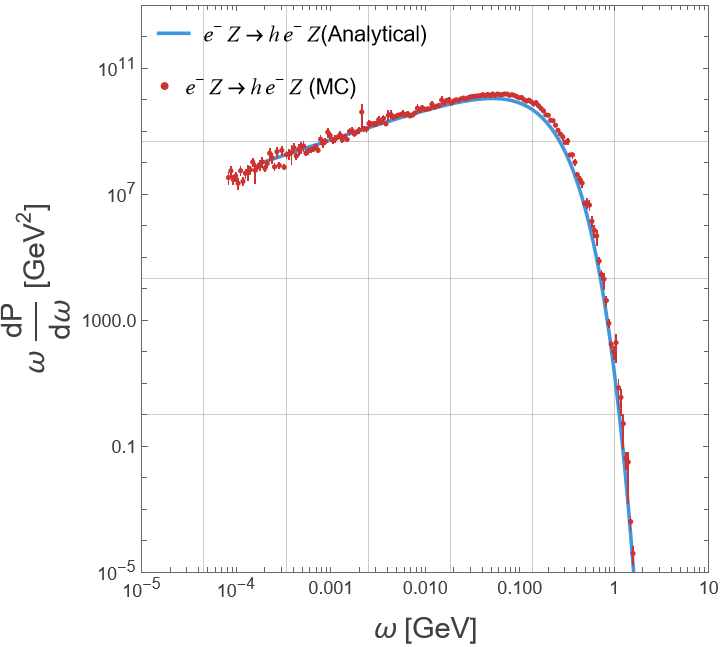
\includegraphics[width=\linewidth]{figures/ez_analytical_mc.png}
    \caption{}
    \label{fig:ez}
  \end{subfigure}

  \caption{
    Analytical and ROOT Monte Carlo results for gravitational
    bremsstrahlung:
    (a) electron--electron bremsstrahlung,
    $e^- e^- \to h e^- e^-$;
    (b) electron--heavy-target bremsstrahlung,
    $e^- Z \to h e^- Z$.
    The Monte Carlo implementation uses the screened leading-soft
    squared amplitudes described in the text.
  }
  \label{fig:bremsstrahlung_validation}
\end{figure}
\FloatBarrier


% ============================================================
% Electron-positron annihilation
% ============================================================
\begin{figure}[H]
  \centering
  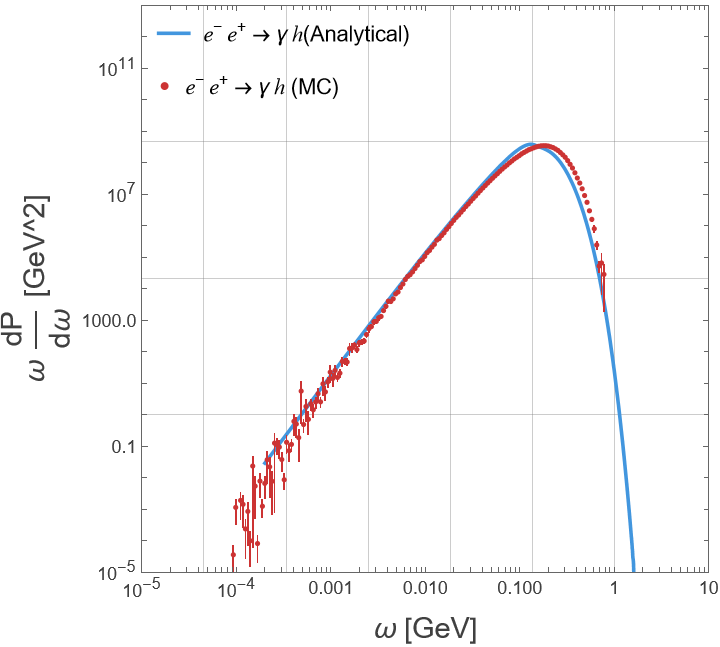
\includegraphics[width=0.52\linewidth]
    {figures/eann_analytical_mc.png}

  \caption{
    Analytical and ROOT Monte Carlo results for electron--positron
    annihilation,
    $e^- e^+ \to h\gamma$.
    The Monte Carlo calculation uses the finite-temperature electron
    chemical potential contained in the dedicated supernova profile.
  }
  \label{fig:eann}
\end{figure}
\FloatBarrier


\section{Operational notes and limitations}

\begin{itemize}
  \item \textbf{Reweighting is essential.} Do not interpret raw ROOT entries as equally weighted physical collisions. Proposal corrections and phase-space weights are part of the integration measure.
  \item \textbf{Use the matching generator and reweighter.} ROOT branches and metadata are channel-specific. A pool from one generator is not interchangeable with another channel's reweighter.
  \item \textbf{Check tail statistics.} A visually noisy low-$\omega$ tail can be caused by small effective weighted counts. Increase proposal statistics or adjust the proposal only after preserving the corresponding importance correction.
  \item \textbf{Keep screening unique.} For bremsstrahlung, do not combine the squared-amplitude screening weights with an effective-mass propagator or a second screening factor.
  \item \textbf{Record run settings.} Preserve the input profile, channel, proposal count, random seed, radius, source revision, and output CSV alongside production results.
  \item \textbf{Separate kinematic exactness from model assumptions.} The ROOT phase-space generation enforces the chosen on-shell final-state kinematics. It does not remove the soft-limit, static-target, massless-electron, screening, or thermal-distribution approximations built into the channel implementation.
\end{itemize}



\end{document}
